\PassOptionsToPackage{unicode=true}{hyperref} % options for packages loaded elsewhere
\PassOptionsToPackage{hyphens}{url}
%
\documentclass[9pt,ignorenonframetext,]{beamer}
\usepackage{pgfpages}
\setbeamertemplate{caption}[numbered]
\setbeamertemplate{caption label separator}{: }
\setbeamercolor{caption name}{fg=normal text.fg}
\beamertemplatenavigationsymbolsempty
% Prevent slide breaks in the middle of a paragraph:
\widowpenalties 1 10000
\raggedbottom
\setbeamertemplate{part page}{
\centering
\begin{beamercolorbox}[sep=16pt,center]{part title}
  \usebeamerfont{part title}\insertpart\par
\end{beamercolorbox}
}
\setbeamertemplate{section page}{
\centering
\begin{beamercolorbox}[sep=12pt,center]{part title}
  \usebeamerfont{section title}\insertsection\par
\end{beamercolorbox}
}
\setbeamertemplate{subsection page}{
\centering
\begin{beamercolorbox}[sep=8pt,center]{part title}
  \usebeamerfont{subsection title}\insertsubsection\par
\end{beamercolorbox}
}
\AtBeginPart{
  \frame{\partpage}
}
\AtBeginSection{
  \ifbibliography
  \else
    \frame{\sectionpage}
  \fi
}
\AtBeginSubsection{
  \frame{\subsectionpage}
}
\usepackage{lmodern}
\usepackage{amssymb,amsmath}
\usepackage{ifxetex,ifluatex}
\usepackage{fixltx2e} % provides \textsubscript
\ifnum 0\ifxetex 1\fi\ifluatex 1\fi=0 % if pdftex
  \usepackage[T1]{fontenc}
  \usepackage[utf8]{inputenc}
  \usepackage{textcomp} % provides euro and other symbols
\else % if luatex or xelatex
  \usepackage{unicode-math}
  \defaultfontfeatures{Ligatures=TeX,Scale=MatchLowercase}
\fi
% use upquote if available, for straight quotes in verbatim environments
\IfFileExists{upquote.sty}{\usepackage{upquote}}{}
% use microtype if available
\IfFileExists{microtype.sty}{%
\usepackage[]{microtype}
\UseMicrotypeSet[protrusion]{basicmath} % disable protrusion for tt fonts
}{}
\IfFileExists{parskip.sty}{%
\usepackage{parskip}
}{% else
\setlength{\parindent}{0pt}
\setlength{\parskip}{6pt plus 2pt minus 1pt}
}
\usepackage{hyperref}
\hypersetup{
            pdftitle={INLA},
            pdfauthor={Tullia Padellini},
            pdfborder={0 0 0},
            breaklinks=true}
\urlstyle{same}  % don't use monospace font for urls
\newif\ifbibliography
\usepackage{color}
\usepackage{fancyvrb}
\newcommand{\VerbBar}{|}
\newcommand{\VERB}{\Verb[commandchars=\\\{\}]}
\DefineVerbatimEnvironment{Highlighting}{Verbatim}{commandchars=\\\{\}}
% Add ',fontsize=\small' for more characters per line
\usepackage{framed}
\definecolor{shadecolor}{RGB}{248,248,248}
\newenvironment{Shaded}{\begin{snugshade}}{\end{snugshade}}
\newcommand{\AlertTok}[1]{\textcolor[rgb]{0.94,0.16,0.16}{#1}}
\newcommand{\AnnotationTok}[1]{\textcolor[rgb]{0.56,0.35,0.01}{\textbf{\textit{#1}}}}
\newcommand{\AttributeTok}[1]{\textcolor[rgb]{0.77,0.63,0.00}{#1}}
\newcommand{\BaseNTok}[1]{\textcolor[rgb]{0.00,0.00,0.81}{#1}}
\newcommand{\BuiltInTok}[1]{#1}
\newcommand{\CharTok}[1]{\textcolor[rgb]{0.31,0.60,0.02}{#1}}
\newcommand{\CommentTok}[1]{\textcolor[rgb]{0.56,0.35,0.01}{\textit{#1}}}
\newcommand{\CommentVarTok}[1]{\textcolor[rgb]{0.56,0.35,0.01}{\textbf{\textit{#1}}}}
\newcommand{\ConstantTok}[1]{\textcolor[rgb]{0.00,0.00,0.00}{#1}}
\newcommand{\ControlFlowTok}[1]{\textcolor[rgb]{0.13,0.29,0.53}{\textbf{#1}}}
\newcommand{\DataTypeTok}[1]{\textcolor[rgb]{0.13,0.29,0.53}{#1}}
\newcommand{\DecValTok}[1]{\textcolor[rgb]{0.00,0.00,0.81}{#1}}
\newcommand{\DocumentationTok}[1]{\textcolor[rgb]{0.56,0.35,0.01}{\textbf{\textit{#1}}}}
\newcommand{\ErrorTok}[1]{\textcolor[rgb]{0.64,0.00,0.00}{\textbf{#1}}}
\newcommand{\ExtensionTok}[1]{#1}
\newcommand{\FloatTok}[1]{\textcolor[rgb]{0.00,0.00,0.81}{#1}}
\newcommand{\FunctionTok}[1]{\textcolor[rgb]{0.00,0.00,0.00}{#1}}
\newcommand{\ImportTok}[1]{#1}
\newcommand{\InformationTok}[1]{\textcolor[rgb]{0.56,0.35,0.01}{\textbf{\textit{#1}}}}
\newcommand{\KeywordTok}[1]{\textcolor[rgb]{0.13,0.29,0.53}{\textbf{#1}}}
\newcommand{\NormalTok}[1]{#1}
\newcommand{\OperatorTok}[1]{\textcolor[rgb]{0.81,0.36,0.00}{\textbf{#1}}}
\newcommand{\OtherTok}[1]{\textcolor[rgb]{0.56,0.35,0.01}{#1}}
\newcommand{\PreprocessorTok}[1]{\textcolor[rgb]{0.56,0.35,0.01}{\textit{#1}}}
\newcommand{\RegionMarkerTok}[1]{#1}
\newcommand{\SpecialCharTok}[1]{\textcolor[rgb]{0.00,0.00,0.00}{#1}}
\newcommand{\SpecialStringTok}[1]{\textcolor[rgb]{0.31,0.60,0.02}{#1}}
\newcommand{\StringTok}[1]{\textcolor[rgb]{0.31,0.60,0.02}{#1}}
\newcommand{\VariableTok}[1]{\textcolor[rgb]{0.00,0.00,0.00}{#1}}
\newcommand{\VerbatimStringTok}[1]{\textcolor[rgb]{0.31,0.60,0.02}{#1}}
\newcommand{\WarningTok}[1]{\textcolor[rgb]{0.56,0.35,0.01}{\textbf{\textit{#1}}}}
\setlength{\emergencystretch}{3em}  % prevent overfull lines
\providecommand{\tightlist}{%
  \setlength{\itemsep}{0pt}\setlength{\parskip}{0pt}}
\setcounter{secnumdepth}{0}

% set default figure placement to htbp
\makeatletter
\def\fps@figure{htbp}
\makeatother

\usetheme{Pittsburgh}
\usecolortheme{seagull}
\usepackage{graphicx}
\usepackage{amsmath}
\usepackage{amsthm}
\usepackage{setspace}
\usepackage{bm}
\usepackage{bbm}
\usepackage{pgf}
\usepackage{caption}
\usepackage{subcaption}
\usepackage{booktabs}
\usepackage{tabularx}
\usepackage{amssymb}
\usepackage{hyperref}
\usepackage{algorithm2e}
\usepackage{mathtools}
\usepackage{multirow}
\usepackage{animate}
\def\labelitemi{\ast}
\definecolor{gray}{RGB}{120,80,10}
\definecolor{red}{RGB}{20,80,100}
\definecolor{light}{RGB}{20,80,100}
\DeclarePairedDelimiter{\ceil}{\lceil}{\rceil}
\setbeamercolor{frametitle}{fg=black}
\setbeamercolor{framesubtitle}{fg=light!80}
\setbeamercolor{structure}{fg=light}
\setbeamertemplate{itemize subitem}{}
\newcommand{\norm}[1]{\left\lVert#1\right\rVert}
\usepackage{blindtext}
\usepackage{tikz}
\usepackage{fontawesome}

\title{INLA}
\author{Tullia Padellini}
\date{}

\begin{document}
\frame{\titlepage}

\begin{frame}

\begin{tikzpicture}[remember picture,overlay] % Background box
\node [xshift=\paperwidth/2,yshift=\paperheight/2] at (current page.south west)[rectangle,fill,inner sep=0pt,minimum width=\paperwidth,minimum height=3*\paperheight/5,top color=light,bottom color=light]{}; % Change the height of the box, its colors and position on the page here
\end{tikzpicture}

\color{white}\sffamily

\hfill \huge{INLA\\ \hfill \Large{as much as you can learn in 90 minutes}}
\vspace{0.6cm}

\begin{columns}

\begin{column}{0.45\textwidth}
\vspace{1.55cm}


\includegraphics[width=.7\textwidth]{sapienza-logo-png-6.png}

{\small Dipartimento di Scienze Statistiche}

\end{column}

\begin{column}{0.45\textwidth}

\hfill \Large{Tullia Padellini}

\vspace{0.25cm}


\hfill \scriptsize{tulliapadellini.github.io     \faLaptop} 

\hfill \scriptsize{tullia.padellini@uniroma1.it   \faEnvelope}

\vspace{0.5cm}
\vspace{0.3cm}




\vspace{0.7cm}
\vfill
\hfill Roma -- 11 December 2019 
\end{column}

\end{columns}

\clearpage

\end{frame}

\begin{frame}[fragile]{INLA}
\protect\hypertarget{inla}{}

\framesubtitle{what are we doing here today}

Efficient (i.e. \emph{fast}) and accurate computational tool for
Bayesian Statistics.

\vspace{.7cm}

\begin{itemize}
\tightlist
\item
  INLA - the method

  \begin{itemize}
  \tightlist
  \item
    a \textbf{deterministic} algorithm to approximate the posterior
    distribution
  \end{itemize}
\end{itemize}

\vspace{0.5cm}

\begin{itemize}
\tightlist
\item
  \texttt{R-INLA} - the implementation

  \begin{itemize}
  \tightlist
  \item
    an \texttt{R} package to perform fit a large class of models in a
    Bayesian way
  \end{itemize}
\end{itemize}

\end{frame}

\begin{frame}[fragile]{INLA -\texttt{I}ntegrated \texttt{N}ested
\texttt{L}aplace \texttt{A}proximation}
\protect\hypertarget{inla--integrated-nested-laplace-aproximation}{}

\framesubtitle{you can have the cake and eat it too}

\begin{itemize}
\tightlist
\item
  \textbf{it's fast}

  \begin{itemize}
  \tightlist
  \item
    relies on numerical approximation and sparse matrices
  \end{itemize}
\end{itemize}

\vspace{0.25cm}

\begin{itemize}
\tightlist
\item
  \textbf{it's accurate}

  \begin{itemize}
  \tightlist
  \item
    empirically shows better performances than MCMC
  \end{itemize}
\end{itemize}

\vspace{0.25cm}

\begin{itemize}
\tightlist
\item
  \textbf{it's flexible}

  \begin{itemize}
  \tightlist
  \item
    can be used to fit any model formulated as a GAN
  \end{itemize}
\end{itemize}

\vspace{0.25cm}

\begin{itemize}
\tightlist
\item
  \textbf{it is} (relatively) \textbf{easy to use}

  \begin{itemize}
  \tightlist
  \item
    it's implemented as an \texttt{R} package
  \end{itemize}
\end{itemize}

\end{frame}

\begin{frame}{Motivation}
\protect\hypertarget{motivation}{}

\framesubtitle{isn't MCMC good enough?}

Do we actually need \textbf{yet another way} to implement Bayesian
Methods?

\vspace{0.25cm}

Yes if we think that MCMC methods are

\begin{itemize}
\tightlist
\item
  cumbersome to write
\item
  slow
\end{itemize}

\vspace{0.25cm}

And this is very much true when dealing with Spatial Models

\end{frame}

\begin{frame}{INLA vs MCMC take I}
\protect\hypertarget{inla-vs-mcmc-take-i}{}

\framesubtitle{MCMC are cumbersome to write}

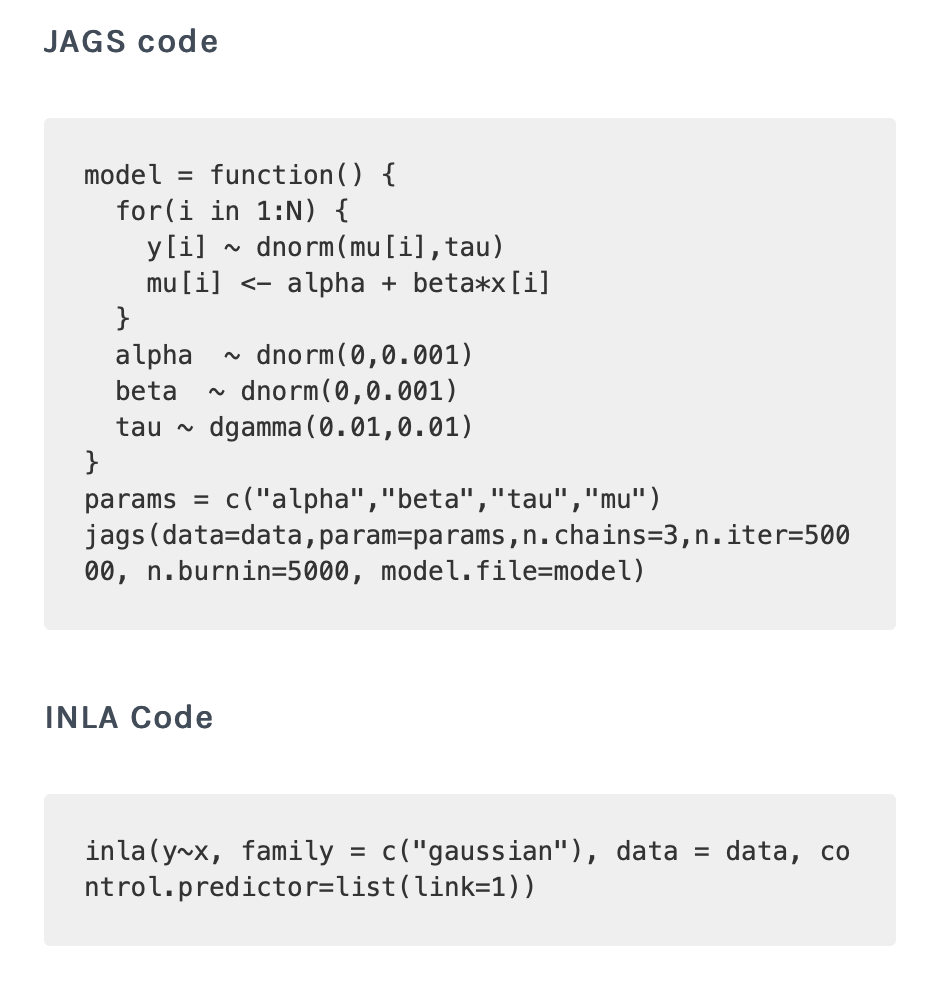
\includegraphics[width=.7\textwidth]{write.png}

\end{frame}

\begin{frame}{INLA vs MCMC take II}
\protect\hypertarget{inla-vs-mcmc-take-ii}{}

\framesubtitle{MCMC are slow}

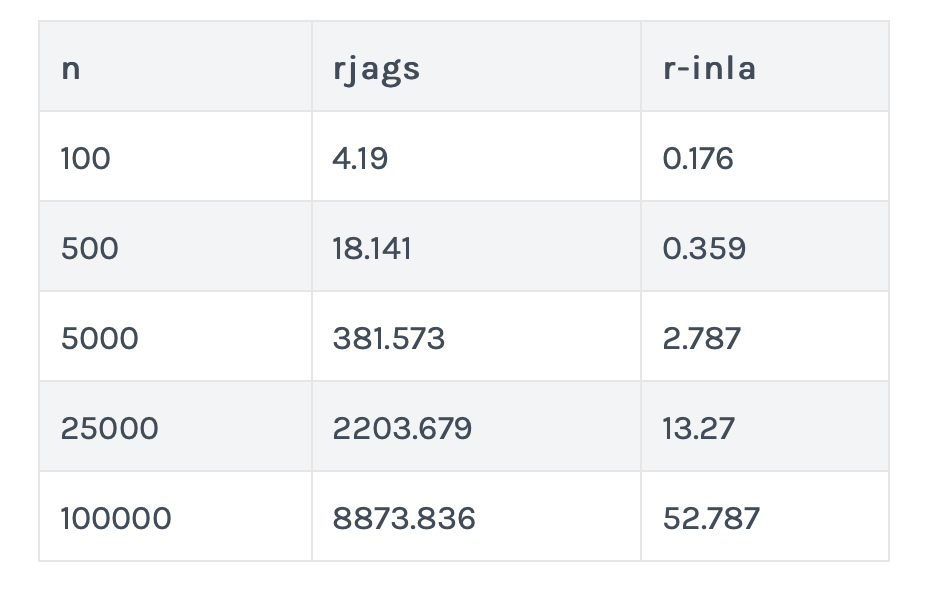
\includegraphics[width=.9\textwidth]{run.png}

\end{frame}

\hypertarget{inla-1}{%
\section{INLA}\label{inla-1}}

\begin{frame}[fragile]{INLA models}
\protect\hypertarget{inla-models}{}

\framesubtitle{basically most of the models you have already seen}

\begin{align*}
    y|\theta, \psi &\sim  \pi(y; \theta, \psi) & & \text{Likelihood}\\
    \theta | \psi &\sim  \only<1>{\pi(\theta;\psi)}\only<2-3>{N(\theta; 0, \Sigma(\psi) )} & & \text{Latent structure }\\
    \psi &\sim \pi(\psi) & & \text{Hyperprior}\\
\end{align*}

\texttt{INLA} provides \textbf{numerical} approximations of the marginal
posteriors \[\pi(\theta_i| y) \qquad \qquad    \pi(\psi_j | y)\]

\pause
\pause

Linear models naturally fall in the \texttt{INLA} framework when we
consider \(\theta = (\beta, f_1, f_2, \dots)\)
\[y= k(\eta) + \epsilon  \qquad \quad \eta = x^t\beta + \sum_k f_k(z_k)\]
where \(\sum_k f_k(z_k)\) can represent random effects, splines,
anything you like.

\end{frame}

\begin{frame}{Laplace Approximation}
\protect\hypertarget{laplace-approximation}{}

\framesubtitle{the basic intuition}

Laplace approximation is based on the following two key idea:

\begin{align*}
f(x) & = \exp[\log(f(x))] \\
g(x) & = g(x^*) + g''(x^*)(x-x^*)^2 + \text{error} \approx g''(x^*)(x-x^*)^2
\end{align*}

So that for every density \(f\) we have
\[f(x) \approx \exp[\log(f)'' (x^*)(x-x^*)^2]\]

\vspace{.5cm}

\pause

Intuitively we can approximate any density \(f\) with a Gaussian by:

\begin{itemize}
\tightlist
\item
  matching the mode to the mean of the Gaussian, \(\mu = x^*\)
\item
  setting the variance by looking at the curvaure at the mode
  \(\sigma = -1/\log(f)''(x^*)\)
\end{itemize}

\end{frame}

\begin{frame}{Basic INLA assumptions}
\protect\hypertarget{basic-inla-assumptions}{}

\framesubtitle{most verbose slide of the day}

\begin{enumerate}
\item
  Each data point depends on only one of the elements in the latent
  Gaussian field \(\theta\), the linear predictor \vspace{.15cm}
\item
  The size of the hyperparameter vector \(\psi\) is small (say
  \textless{} 15) \vspace{.15cm}
\item
  The latent field \(\theta\), can be large but it is endowed with some
  conditional independence (Markov) properties so that the precision
  matrix \(\Sigma^{-1}(\psi)\) is sparse. \vspace{.15cm}
\item
  The linear predictor depends linearly on the unknown smooth function
  of covariates. \vspace{.15cm}
\item
  The inferential interest lies in the univariate posterior marginals
  \(\pi(\theta_i|y)\) and \(\pi(\psi_j|y)\) rather than in the joint
  posterior \(\pi(\theta, \psi|y)\).
\end{enumerate}

\end{frame}

\begin{frame}{INLA}
\protect\hypertarget{inla-2}{}

\framesubtitle{it's time for the formulas}

\begin{align*}
\pi(\theta_i|y) & = \int \int \pi(\theta, \psi|y) d\theta_{-i} d\psi = \int \textcolor<3->{red}{\pi(\theta_{i}|\psi,y)} \textcolor<2->{gray}{\pi(\psi|y)}d\psi \\
\only<2->{\widehat{\pi}(\theta_i|y) & = \sum_{k} \textcolor<3->{red}{\widehat{\pi}(\theta_{i}|\psi^{(k)},y)} \textcolor<2->{gray}{\widehat{\pi}(\psi^{(k)}|y)}\Delta^{(k)}}
\end{align*}

\pause

\vspace{0.75cm}

\begin{itemize}[<+->]
\tightlist
\item
  Approximate \(\textcolor{gray}{\pi(\psi|y)}\) and
  \(\textcolor{red}{\pi(\theta_{i}|\psi,y)}\) through Laplace
  Approximation
\item
  Approximate the integrals over \(\psi\) with summations over a finite
  set of values \(\psi^{(1)},\dots, \psi^{(K)}\)
\end{itemize}

\end{frame}

\begin{frame}{Back to our Basic INLA assumptions}
\protect\hypertarget{back-to-our-basic-inla-assumptions}{}

\framesubtitle{still most verbose slide of the day}

\begin{enumerate}
\item
  Each data point depends on only one of the elements in the latent
  Gaussian field \(\theta\), the linear predictor \vspace{.15cm}
\item
  \textcolor{gray}{The size of the hyperparameter vector $\psi$ is small (say < 15)}
  \vspace{.15cm}
\item
  The latent field \(\theta\), can be large but it is endowed with some
  conditional independence (Markov) properties so that the precision
  matrix \(\Sigma^{-1}(\psi)\) is sparse. \vspace{.15cm}
\item
  The linear predictor depends linearly on the unknown smooth function
  of covariates. \vspace{.15cm}
\item
  \textcolor{gray}{The inferential interest lies in the univariate posterior marginals $\pi(\theta_i|y)$ and $\pi(\psi_j|y)$ rather than in the joint posterior $\pi(\theta, \psi|y)$.}
\end{enumerate}

\end{frame}

\begin{frame}{Posterior of \(\psi\)}
\protect\hypertarget{posterior-of-psi}{}

\framesubtitle{starting from the ``deepest'' level}

\[ \pi(\psi|y) = \frac{\pi(\theta, \psi|y)}{\pi(\theta | \psi, y)} \textcolor<1>{white}{\propto \frac{\pi(y| \theta, \psi) \pi(\theta | \psi) \pi(\psi)}{\pi(\theta | \psi, y)}}\]

\pause

\vspace{0.5cm}

Here comes the \textbf{Laplace approximation:}

Approximate \(\pi(\theta | \psi, y)\) with a Gaussian
\(\widehat{\pi}_G(\theta | \psi, y) = N(\theta; \mu, Q^{-1})\) wherer

\begin{itemize}
\tightlist
\item
  \(\mu\) is the mode of \(\pi(\theta | \psi, y)\)
\item
  \(-Q\) is the curvature of \(\log[\pi(\theta | \psi, y)]\) at the mode
  \(\mu\)
\end{itemize}

\pause

\[ \widehat{\pi}(\psi|y) = \frac{\pi(\theta, \psi|y)}{\widehat{\pi}_G(\theta | \psi, y)} {\propto \frac{\pi(y| \theta, \psi) \pi(\theta | \psi) \pi(\psi)}{\widehat{\pi}_G(\theta | \psi, y)}}\]

\end{frame}

\begin{frame}{INLA}
\protect\hypertarget{inla-3}{}

\framesubtitle{and we are back here}

\begin{align*}
\pi(\theta_i|y) & = \int \int \pi(\theta, \psi|y) d\theta_{-i} d\psi = \int \textcolor{red}{\pi(\theta_{i}|\psi,y)} \textcolor{gray}{\pi(\psi|y)}d\psi
\end{align*}

\vspace{0.5cm}

\begin{itemize}
\tightlist
\item
  Approximate \(\textcolor{gray}{\pi(\psi|y)}\) and
  \(\textcolor{red}{\pi(\theta_{i}|\psi,y)}\) through Laplace
  Approximation
\item
  Approximate the integrals over \(\psi\) with summations over a set of
  \emph{carefully chosen} values \(\psi^{(1)},\dots, \psi^{(K)}\)
\end{itemize}

\vspace{0.5cm}

\begin{align*}
\widehat{\pi}(\theta_i|y) & = \sum_{k} \textcolor{red}{\widehat{\pi}(\theta_{i}|\psi^{(k)},y)} \textcolor{gray}{\widehat{\pi}(\psi^{(k)}|y)}\Delta^{(k)}
\end{align*}

\end{frame}

\begin{frame}{Approximate the Posterior Latent Field}
\protect\hypertarget{approximate-the-posterior-latent-field}{}

\framesubtitle{skipping all the details}

\[ \pi(\theta_i|\psi, y) = \frac{\pi(\theta| \psi, y)}{\pi(\theta_{-i} |\theta_i, \psi, y)} \textcolor<1>{white}{\propto \frac{\pi(y|\theta, \psi)\pi(\theta|\psi)\pi(\psi)}{\pi(\theta_{-i} |\theta_i, \psi, y)}}\]

\pause

\vspace{0.5cm}

\begin{itemize}
\tightlist
\item
  \textbf{Gaussian}: use the marginals of
  \(\widehat{\pi}_G(\theta | \psi, y)\) computed before
\item
  \textbf{Laplace approximation}: use a Gaussian approximation for the
  denominator \(\pi(\theta_{-i} |\theta_i, \psi, y)\)
\item
  \textbf{Simplified Laplace approximation}: a mix of the two
\end{itemize}

\end{frame}

\begin{frame}{Putting everything together}
\protect\hypertarget{putting-everything-together}{}

\begin{enumerate}
\item
  Explore the space of \(\psi\) through the approximation
  \(\widehat{\pi}(\psi|y)\). \vspace{0.15cm}

  \begin{itemize}
  \tightlist
  \item
    Find the mode of \(\widehat{\pi}(\psi|y)\)
  \item
    Select \({\psi^{(1)}, \dots, \psi^{(K)}}\) in the area of high
    density of \(\widehat{\pi}(\psi|y)\) \vspace{0.25cm}
  \end{itemize}
\item
  Compute \(\widehat{\pi}(\psi^{(k)}|y)\) for each
  \({\psi^{(1)}, \dots, \psi^{(K)}}\) \vspace{0.25cm}
\item
  Compute \(\widehat{\pi}(\theta_i|\psi^{(k)},y)\) for each
  \({\psi^{(1)}, \dots, \psi^{(K)}}\) \vspace{0.25cm}
\item
  Approximate \(\pi(\theta_i|y)\) as
  \[\widehat{\pi}(\theta_i|y) = \sum_{k} \textcolor{red}{\widehat{\pi}(\theta_{i}|\psi^{(k)},y)} \textcolor{gray}{\widehat{\pi}(\psi^{(k)}|y)}\Delta^{(k)}\]
\end{enumerate}

\end{frame}

\hypertarget{r-inla}{%
\section{R-INLA}\label{r-inla}}

\begin{frame}[fragile]{Installation}
\protect\hypertarget{installation}{}

\framesubtitle{it is non-trivial already}

INLA is not on CRAN, so you need to specify the repository when you
install it:

\vspace{0.75cm}

\begin{Shaded}
\begin{Highlighting}[]
\KeywordTok{install.packages}\NormalTok{(}\StringTok{"INLA"}\NormalTok{, }
                 \DataTypeTok{repos =} \StringTok{"https://inla.r-inla-download.org/R/stable"}\NormalTok{, }
                 \DataTypeTok{dep =} \OtherTok{TRUE}\NormalTok{)}
\end{Highlighting}
\end{Shaded}

\vspace{0.25cm}

\texttt{INLA} gets constant updating - check your version

\end{frame}

\begin{frame}[fragile]{Setting up the model}
\protect\hypertarget{setting-up-the-model}{}

\framesubtitle{building blocks of the \texttt{inla} call}

The generic \texttt{inla} call is structured as follows:

\begin{Shaded}
\begin{Highlighting}[]
\KeywordTok{inla}\NormalTok{(formula, data, family)}
\end{Highlighting}
\end{Shaded}

\vspace{0.25cm}

\begin{itemize}
\item
  \texttt{formula}: formula object that specifies the linear predictor
\item
  \texttt{data}: data frame with the data
\item
  \texttt{family}: string that indicate the likelihood family (default
  is Gaussian)
\end{itemize}

\end{frame}

\begin{frame}[fragile]{Toy Example}
\protect\hypertarget{toy-example}{}

\framesubtitle{most famous dataset ever}

The basic formulation of a linear regression model is almost the same as
the canonical \texttt{lm} function:

\begin{Shaded}
\begin{Highlighting}[]
\KeywordTok{library}\NormalTok{(INLA)}

\KeywordTok{data}\NormalTok{(iris)}

\NormalTok{mod1  =}\StringTok{ }\KeywordTok{inla}\NormalTok{(Petal.Length }\OperatorTok{~}\StringTok{ }\DecValTok{1} \OperatorTok{+}\StringTok{ }\NormalTok{Petal.Width, }\DataTypeTok{data =}\NormalTok{ iris)}

\NormalTok{mod1_lm =}\StringTok{ }\KeywordTok{lm}\NormalTok{(Petal.Length }\OperatorTok{~}\StringTok{ }\DecValTok{1} \OperatorTok{+}\StringTok{ }\NormalTok{Petal.Width, }\DataTypeTok{data =}\NormalTok{ iris)}
\end{Highlighting}
\end{Shaded}

\end{frame}

\begin{frame}[fragile]{The \texttt{formula} argument}
\protect\hypertarget{the-formula-argument}{}

\framesubtitle{how to specify the model components}

The formula object specifies the building blocks of the linear predictor

\[y= k(\eta) + \epsilon  \qquad \quad \eta = x^t\beta + \sum_k f_k(z_k)\]

\begin{verbatim}
formula = y ~ x + f(id, model)
\end{verbatim}

\vspace{0.25cm}

The \texttt{f} terms contains random effect

\begin{itemize}
\tightlist
\item
  \texttt{id} name of the variable
\item
  \texttt{model} name of the model of the random effect corresponding to
  \texttt{id}
\end{itemize}

\end{frame}

\begin{frame}[fragile]{Toy Example}
\protect\hypertarget{toy-example-1}{}

\framesubtitle{most famous dataset ever}

\begin{Shaded}
\begin{Highlighting}[]
\NormalTok{formula =}\StringTok{ }\NormalTok{Petal.Length }\OperatorTok{~}\StringTok{ }\DecValTok{1} \OperatorTok{+}\StringTok{ }\NormalTok{Petal.Width }\OperatorTok{+}\StringTok{ }\KeywordTok{f}\NormalTok{(Species, }\DataTypeTok{model =} \StringTok{"iid"}\NormalTok{)}

\NormalTok{mod2=}\StringTok{ }\KeywordTok{inla}\NormalTok{(formula, }\DataTypeTok{data =}\NormalTok{ iris)}
\end{Highlighting}
\end{Shaded}

\vspace{0.25cm}

\textbf{NB:} The list of all possible latent models can be found using:

\begin{Shaded}
\begin{Highlighting}[]
\KeywordTok{names}\NormalTok{(}\KeywordTok{inla.models}\NormalTok{()}\OperatorTok{$}\NormalTok{latent)}
\KeywordTok{inla.doc}\NormalTok{(}\StringTok{"ar1"}\NormalTok{)}
\end{Highlighting}
\end{Shaded}

\end{frame}

\begin{frame}[fragile]{The \texttt{data} argument}
\protect\hypertarget{the-data-argument}{}

\framesubtitle{how to input the observations to `inla`}

Data are typically provided through a \texttt{data.frame} (although
named \texttt{list} can also be used).

\vspace{0.25cm}

\begin{itemize}
\item
  If the response is a factor it must be converted to \{0, 1\} before
  calling \texttt{inla()}, as this conversion is not done automatic (as
  for example in \texttt{glm()}). \vspace{0.15cm}
\item
  If the covariate is binary it has to be converted to a
  \texttt{factor}, otherwise inla will treat it as numeric
  \vspace{0.15cm}
\item
  If we wish to predict the response variable for some observations, we
  need to specify the response variable of these observations as
  \texttt{NA}
\end{itemize}

\end{frame}

\begin{frame}[fragile]{The \texttt{family} argument}
\protect\hypertarget{the-family-argument}{}

\framesubtitle{how to specify the likelihood}

The family argument is a string defining the likelihood of our model.

\begin{itemize}
\item
  each observation can have a different likelihood: vector of strings
  that indicate the likelihood family
\item
  depending on the likelihood we are using, we may have additional
  arguments to provide to the \texttt{inla()} call
\end{itemize}

\begin{Shaded}
\begin{Highlighting}[]
\KeywordTok{inla}\NormalTok{(formula, data, }\DataTypeTok{family =} \StringTok{"binomial"}\NormalTok{, Ntrials)}
\end{Highlighting}
\end{Shaded}

\begin{itemize}
\tightlist
\item
  we may have more than one link function corresponding to each family
  (as in the \texttt{logit} or \texttt{probit} case).
  \texttt{control.family=list(control.link=list(model="model")))}
\end{itemize}

\vspace{0.15cm}

\textbf{NB:} The list of all possible likelihoods can be found using:

\begin{Shaded}
\begin{Highlighting}[]
\KeywordTok{names}\NormalTok{(}\KeywordTok{inla.models}\NormalTok{()}\OperatorTok{$}\NormalTok{link)}
\end{Highlighting}
\end{Shaded}

\end{frame}

\begin{frame}[fragile]{Toy Example}
\protect\hypertarget{toy-example-2}{}

\framesubtitle{most famous dataset ever}

\begin{Shaded}
\begin{Highlighting}[]
\KeywordTok{data}\NormalTok{(}\StringTok{"Seeds"}\NormalTok{)}

\NormalTok{res =}\StringTok{ }\KeywordTok{inla}\NormalTok{(}\DataTypeTok{formula=}\NormalTok{ r }\OperatorTok{~}\StringTok{ }\NormalTok{x1 }\OperatorTok{+}\StringTok{ }\NormalTok{x2, }\DataTypeTok{data =}\NormalTok{ Seeds,}
           \DataTypeTok{family =} \StringTok{"binomial"}\NormalTok{, }\DataTypeTok{Ntrials =}\NormalTok{ n,}
           \DataTypeTok{control.family =} \KeywordTok{list}\NormalTok{(}\DataTypeTok{control.link=}\KeywordTok{list}\NormalTok{(}\DataTypeTok{model =} \StringTok{"logit"}\NormalTok{)))}
\KeywordTok{summary}\NormalTok{(res)}
\end{Highlighting}
\end{Shaded}

\vspace{0.75cm}

To see all available likelihood and links you can use:

\begin{Shaded}
\begin{Highlighting}[]
\KeywordTok{names}\NormalTok{(}\KeywordTok{inla.models}\NormalTok{()}\OperatorTok{$}\NormalTok{link)}
\KeywordTok{names}\NormalTok{(}\KeywordTok{inla.models}\NormalTok{()}\OperatorTok{$}\NormalTok{likelihood)}
\end{Highlighting}
\end{Shaded}

\end{frame}

\begin{frame}[fragile]{Additional Arguments}
\protect\hypertarget{additional-arguments}{}

\begin{itemize}
\tightlist
\item
  \texttt{control.compute}: list with the specification of several
  computing variables such as dic which is a Boolean variable indicating
  whether the DIC of the model should be computed
\end{itemize}

\begin{Shaded}
\begin{Highlighting}[]
\NormalTok{res =}\StringTok{ }\KeywordTok{inla}\NormalTok{(Petal.Length }\OperatorTok{~}\StringTok{ }\DecValTok{1} \OperatorTok{+}\StringTok{ }\NormalTok{Petal.Width, }\DataTypeTok{data =}\NormalTok{ iris,}
            \DataTypeTok{control.compute =} \KeywordTok{list}\NormalTok{(}\DataTypeTok{dic =} \OtherTok{TRUE}\NormalTok{))}
\end{Highlighting}
\end{Shaded}

\begin{itemize}
\tightlist
\item
  \texttt{control.predictor}: list with the specification of several
  predictor variables such as link which is the link function of the
  model, and compute which is a Boolean variable that indicates whether
  the \textcolor<2>{gray}{marginal} densities for the linear predictor
  should be computed.
\end{itemize}

\begin{Shaded}
\begin{Highlighting}[]
\NormalTok{res =}\StringTok{ }\KeywordTok{inla}\NormalTok{(Petal.Length }\OperatorTok{~}\StringTok{ }\DecValTok{1} \OperatorTok{+}\StringTok{ }\NormalTok{Petal.Width, }\DataTypeTok{data =}\NormalTok{ iris,}
           \DataTypeTok{control.predictor =} \KeywordTok{list}\NormalTok{(}\DataTypeTok{compute =} \OtherTok{TRUE}\NormalTok{))}
\end{Highlighting}
\end{Shaded}

\pause

\end{frame}

\begin{frame}[fragile]{Even more additional arguments}
\protect\hypertarget{even-more-additional-arguments}{}

\begin{itemize}
\item
  \texttt{inla.emarginal()} and \texttt{inla.qmarginal()} calculate the
  expectation and quantiles, respectively, of the posterior marginals
  \vspace{0.25cm}
\item
  \texttt{inla.smarginal()} can be used to obtain a spline smoothing of
  the whole marginal \vspace{0.25cm}
\item
  \texttt{inla.tmarginal()} can be used to transform the marginals
  \vspace{0.25cm}
\item
  \texttt{inla.zmarginal()} provides summary statistics \vspace{0.25cm}
\item
  \texttt{inla.dmarginal()} computes the density at particular values
\end{itemize}

\end{frame}

\end{document}
